\section{Design Flow}
\label{sec:design-flow}

We propose a novel design flow for aspect-driven compilation of
dataflow designs to meet the following requirements and design goals,
addressing key areas in developing hardware acceleration solutions:
\begin{enumerate}
\item \emph{Performance:} specify high-performance dataflow designs,
  that achieve significant speedup over sequentially executed
  implementations; exploit the run-time reconfiguration capability of
  FPGA devices to improve performance and efficiency;
\item \emph{Portability:} improve portability of dataflow designs, to
  allow reuse of optimisation strategies on various platforms;
\item \emph{Integration:} simplify translation of existing
  applications to high-performance dataflow designs to facilitate the
  integration of the proposed design flow with existing (predominantly
  imperative) application code;
\item \emph{Productivity:} improve developer productivity by providing
  high-level means of specifying dataflow designs, controlling
  compilation strategies to reduce compilation time and generating
  boilerplate code automatically.
\end{enumerate}

To meet these requirements we propose the following approach. Firstly,
we introduce \MAXC{} (described in Section \ref{sec:maxc}), a novel
language for specifying dataflow designs that provides support for
run-time reconfiguration. We specify the accelerated portion of the
original applications using \MAXC{} dataflow kernels. By maintaining
compatibility with C99 syntax we improve developer productivity by
providing a familiar language and introduce the possibility of
combining hardware and software specifications. Secondly, by using an
aspect driven compilation flow we decouple optimisation from design
development, improving design portability, and we automate the
generation of code and design space exploration improving
productivity. Finally, systematic design space exploration is used to
identify maximum performance configurations, subject to platform
specific constraints.

The proposed design flow is illustrated in Fig.~\ref{fig:design-flow}
and follows the steps: (i) a C application containing an embedded
high-level dataflow design is developed from the original source
application (implemented using \MAXC{}, described in Section
\ref{sec:maxc}), (ii) the dataflow design is transformed
(\emph{woven}) by the aspects in the repository to generate new
designs (e.g with support for run-time reconfiguration, with various
word-length configurations and various compilation times -- these are
covered in detail in Section \ref{sec:aspects}), (iii) the generated
configurations are compiled using a backend compilation toolchain
(currently MaxCompiler) to dataflow designs implemented on FPGAs, (iv)
the feedback from the compilation process is used to drive the design
space exploration, repeating the weaving and compilation process until
user specified requirements are met.

\begin{figure}[!h]
  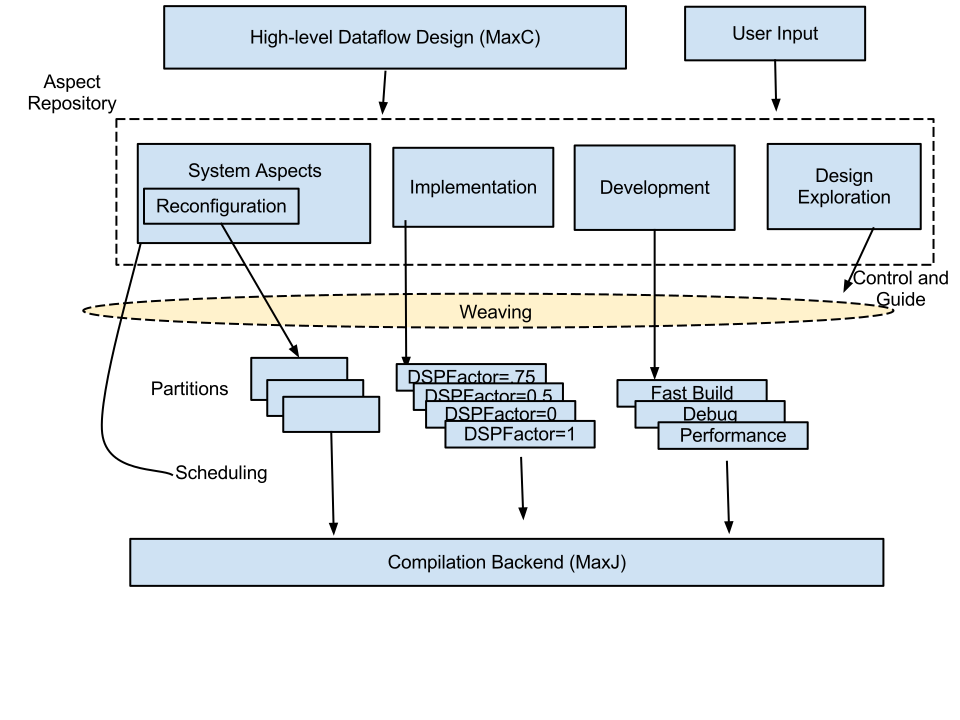
\includegraphics[scale=0.48, trim=60 50 0 0]{figs/design-flow}
  \caption{Proposed approach for aspect-driven compilation of dataflow
    designs.}
  \label{fig:design-flow}
\end{figure}

Compared to existing work described in
\cite{Cardoso:Teixeira:Alves:Nobre:Diniz:Cutinho:Luk:2012} and
\cite{cardoso2011new} our approach emphasises and provides more
freedom in the exploration of design level optimisation (such as word
length optimisations and mapping of arithmetic blocks to DSPs) by
using a combination of implementation aspects (shown in
Fig.~\ref{fig:design-flow}) and \MAXC{} optimisation options.
Additionally our approach targets a dataflow architecture as opposed
to the von Neumann architecture (GPP + Custom accelerator) proposed in
the related work. We explicitly consider and implement run-time
reconfiguration to achieve performance improvements.
